\documentclass[sigconf]{acmart}

\usepackage{hyperref}

\usepackage{endfloat}
\renewcommand{\efloatseparator}{\mbox{}} % no new page between figures

\usepackage{booktabs} % For formal tables
\graphicspath{ {images/} }

\settopmatter{printacmref=false} % Removes citation information below abstract
\renewcommand\footnotetextcopyrightpermission[1]{} % removes footnote with conference information in first column
\pagestyle{plain} % removes running headers

\begin{document}
\title{Using Big Data to minimize Fraud, Waste, and Abuse (FWA) in United States Healthcare}


\author{Paul Marks}
\affiliation{%
  \institution{Indiana University}
  \streetaddress{Online Student}
  \city{Shepherdsville} 
  \state{Kentucky} 
  \postcode{40165}
}
\email{pcmarks@iu.edu}


\begin{abstract}
The cost of healthcare includes the cost of inefficient services.  While this 
could include topics such as misdiagnosis, less effective treatment plans, 
and more efficient use of types of services (emergency room vs. immediate care 
vs. telemedicine) the purpose of this paper is the cost of Fraud, Waste, and 
Abuse (FWA) within the system.  The question is "How can we use big data analysis to 
help minimize these costs and thus optimize the money spent on healthcare."
\end{abstract}

\keywords{i523, hid327, Fraud, Waste, Abuse, Healthcare, Medicare, Medicaid, 
FWA, health insurance}


\maketitle

\section{Introduction}

FWA is all of our issue since healthcare services are leveraged by everyone at some 
point and the costs for those services include the money lost to FWA.  The three 
components of Fraud, Waste and Abuse are varying degrees of culpability.  
The Centers for Medicare and Medicaid Services (CMS) in part defines fraud as 
"knowingly and willfully executing, or attempting to execute, a scheme or artifice 
to defraud any health care benefit program", Waste as "overusing services, or other 
practices that, directly or indirectly, result in unnecessary costs", and Abuse as 
"involves payment for items or services when there is not legal entitlement to that 
payment and the provider has not knowingly and/or intentionally misrepresented 
facts"\cite{MLNFWA}.  While the percentage of cost attributable to FWA
can vary from insurer to insure, Medicare estimates that 11 percent
of its payments for Original Medicare are improper primarily due
to FWA.\cite{FY2016HHSFR}  In combination these cost the United States healthcare system 
80 billion dollars\cite{HFMA} annually.  

Advances in big data technology can help reduce these losses.  Big data offers the 
ability to look at data in real time to determine if a claim is legitimate or not.  
Historically, due to the amount of data involved, this type of analysis would have to 
happen after the claims have been paid with specific models targeting specific 
schemes to identify FWA.  Big data can help lower the cost of health-care in the 
United States by identifying FWA claims and stopping payment before it occurs. 


\section{Healthcare Fraud, Waste, and Abuse Environment}

It is easy to understand the problem FWA poses.  Healthcare funds are of limited 
quantity.  Insurance helps to spread the cost among groups of people, but does not 
provide limitless funds.  As costs increase, so do premiums or direct payments for 
health-care.  In order for as many people to be able to have access to healthcare 
costs have to be managed.  There are many ideas for helping to provide affordable 
healthcare, but there is much discussion and disagreement on exactly how to do that.  
Reducing costs by eliminating as much FWA as possible is one solution that everyone, 
except for those participating in and profiting from FWA schemes, can agree on.

Data to fight FWA is not just the information gathered by a doctor or other provider 
while working with a patient.  In order to fully utilize advances in technology, 
multiple sources of information must be brought together.  Sources include claims 
(current and historic), clinical, provider, geospatial, and other sources of 
information.  This allows for data analytics to take a deeper look into not only a 
single participant, but others who may be related to that participant.  "If Provider 
A is involved in improper billing, it is not uncommon for other providers with which 
they associate to also be engaged in bad behavior.  Thus, many payers will work to 
analyze connected providers.  Information on corporate ownership, billing and 
management companies, social media interactions of physicians and staff can reveal 
whether other physicians, pharmacies, radiology centers, home infusion agencies, etc. 
are engaged in a broader pattern of referral and collusion."\cite{RevCycle}

The problem for big data to solve is the deluge of information and how to process it 
fast enough.  Using CMS as an example, being a government entity much of their data is 
available publicly, it is easy to get an idea of the amount of data.  Medicare processed 
1.2 billion claims in 2014, covering 53.8 million beneficiaries, with 6,142 million 
hospitals, and 1,173,802 non-institutional providers\cite{2015CMSStatistics}.  Payments 
are generally made within a specific timeframe depending on the insurer and their 
agreement with providers.  This time includes all the normal steps to verify and process 
a claim so the time available to examine the data for FWA is very limited.


\subsection{Big Data Techniques for FWA}

So how can big data be used to approach this issue?  Leveraging big data tools such as 
Hadoop analysts could divide the different sources of information into data lakes, 
looking at each source separately, and then combining the results.  Table 
\ref{fig:TypesofFraud} on page \pageref{fig:TypesofFraud} shows sources of information 
and what level of FWA they are generally related to.  The highest level combines sets 
of data.  "Level 7 combines all previous data views and concerns all fraud that is part 
of criminal networks which involve many different beneficiaries and/or providers. This 
much larger data view, spanning billions of claims in the case of Medicaid, is the most 
rich, delivering the ability to perform complex network analysis that could detect 
intricate conspiracies. However, performance of analysis here will be much lower than 
in previous levels."\cite{THORNTON20131252} 

Traditionally programs are written to look for specific sets of circumstances.  
Leveraging existing knowledge about the data and using it to look for specific patterns 
is known as supervised in big data terms.  "There are several supervised fraud detection 
methods such as: Bayesian Networks, Neural Networks (NNs), Decision Trees, and Fuzzy 
Logic. NNs and decision trees are the most popular fraud detection methods because of 
their high tolerance of noisy data and huge data set handling."  There are also 
unsupervised methods in which data is fed into the system without preexisting notions 
of what to look for\cite{Ghuse}.  Unsupervised methods sort through data and find 
relationships and groupings of related information, find clusters of what could be 
considered normal, and determine where the outliers are.  

Applying unsupervised methods to healthcare data will identify patterns that will then 
have to be verified as FWA or acceptable patterns.  "Patrick McIntyre, SVP of Health Care 
Analytics at Anthem, one of the country's biggest payers, credits machine learning and 
big data with their ability to "identify potentially fraudulent or wasteful claims on a 
daily basis." The algorithms are run at the same time as claims are batch processed, so 
questionable claims are immediately identified, flagged and sent to the clinical coding 
experts for review."\cite{Datameer}  This greatly increases the ability to fight FWA by 
having the machine pinpoint where to look in all the data available.  Suddenly the task 
of finding fraud is not as daunting.  By leveraging both of these techniques FWA can be 
discovered at an accelerated pace.  The number of models the system knows will grow over 
time as more data is fed into it and more patters are discovered and verified.

Some fraud schemes can be particularly hard to find.  There are simple cases which follow 
a typical known pattern.  However this is only a portion of the problem.  Fraud schemes 
change and can involve many different entities which may not seem to be related on the 
surface.  The more data which can be combined and analyzed, the more fraud that can be 
found.  "Much of the FWA that plague health care payers is the result of organized, 
sophisticated and collusive activities among providers and between providers and patients. 
Social network analysis can help identify relationships, links and hidden patterns of 
information sharing and interactions within potentially fraudulent clusters, including:
\begin{itemize}
  \item Patient relationships with known perpetrators of health care fraud;
  \item Links between recipients, businesses, assets and relatives and associates;
  \item Links between licensed and non-licensed and sanctioned providers; and
  \item Inappropriate relationships between patients, providers, employees, suppliers 
  and partners"\cite{LexisNexis}
\end{itemize}
In order to keep up with organized fraud activities, there must be a dedicated practice 
of data analytics which is ever evolving. 


\subsection{Future uses of Big Data Analytics}

Currently there is still a certain amount of honor built into healthcare.  "The system's 
inherent structure of trust enables both simple billings errors and illicit actors to hide 
in the shadows of the murky deep as overpayments quietly siphon money away from legitimate 
care."\cite{RevCycle}  If a claim is submitted by a valid entity, using the correct process, 
and everything is in order then it is most likely paid.  For many claims this is done 
without any specific proof of the services being provided.  With more and more healthcare 
information being digitized this may not be the case in the future.  X-rays, lab tests, 
clinical notes, etc. are all being stored digitally.  Computers are now able to interpret 
images and unstructured text very accurately.  By linking this data to claims data the clinical 
information could be required as part of claims payment.  An x-ray of broken bone, notes which 
support a diagnosis, Magnetic Resonance Imaging files, could all be interpreted automatically.  
Not only would the data be used to compare to the claims information, but to other images/notes 
on file to ensure that the same files were not being submitted with multiple claims.  The system 
could know what one individual medical history looks like compared to another similar to how 
facial recognition is able to match like images.  Requiring and being able to validate more 
information before services are paid for would help the reduce the ability of perpetrators of FWA 
to be able to get reimbursed for services they should not.  This level of verification would not 
be possible without the ability to process massive amounts of data quickly.  


Historically the payers of most healthcare claims, insurers, have not had the 
ability to examine actual evidence that a service has taken place on a broad scale.  (It is done 
manually on a specific case or audit basis.)  Through the use of advances in big data and combining 
current and new data stores such as electronic health records into the payment process a difference 
can be made in the amount of money lost to FWA in healthcare.  "By combining identity and entity resolution, 
rules-based claim and clinical review, complex linking analysis and predictive analytics into a 
seamless workflow, we will come closer to migrating an integrated pre-pay fraud solution to a real 
risk control environment with the potential to eliminate billions of dollars in improper payments due 
to FWA. This is not just a health care imperative, but a national economic imperative that must be 
addressed immediately. The analytics exist. It is time for those analytics to be implemented and the 
hard choices that enable that implementation to be made to insure that we remain at the forefront of 
quality care for all Americans."\cite{LexisNexis}


\section{Conclusions}

While there may be disagreement on many aspects of healthcare in America, everyone should agree 
that eliminating Fraud, Waste, and Abuse within the system is the right thing to do.  FWA costs 
billions of dollars annually.  Just a 1 percent reduction in the estimated 80 billion dollars 
annually would result in 800 million dollars in savings.  With this amount of money at stake 
significant investments should continue to be made in leveraging advanced big data technologies 
into solving this problem.  Due to the continued rise in the amount of data collected traditional 
programming cannot keep up with the pace.  Advanced techniques must be leveraged which can learn 
in an unsupervised manner.  The future of the best methods for fighting FWA in healthcare will be 
a combination of this analysis and teams specializing in the rules and regulations of healthcare
in the United States.  The unsupervised methods will work through massive amounts of structured and 
unstructured data breaking it down into cases and schemes which are most like FWA.  These will be 
reviewed, confirmed or denied as accurate, and fed back into overall FWA platform.  As this cycle 
continues over and over the ability to fight FWA in United States Healthcare will get better.  
While Big Data may never eliminate FWA in Healthcare it can help to minimize it and save the
country billions of dollars a year.

\begin{acks}

  The author would like to thank Dr. Gregor von Laszewski for his
  support and suggestions to write this paper.  It has helped to expand my knowledge in how modern 
  data analytics can help to save waste which has plagued the healthcare system.

\end{acks}

\bibliographystyle{ACM-Reference-Format}
\bibliography{report} 

\begin{table}[htb]
    \caption{Types of Fraud and their related Sources\cite{THORNTON20131252}}
    \label{fig:TypesofFraud}
    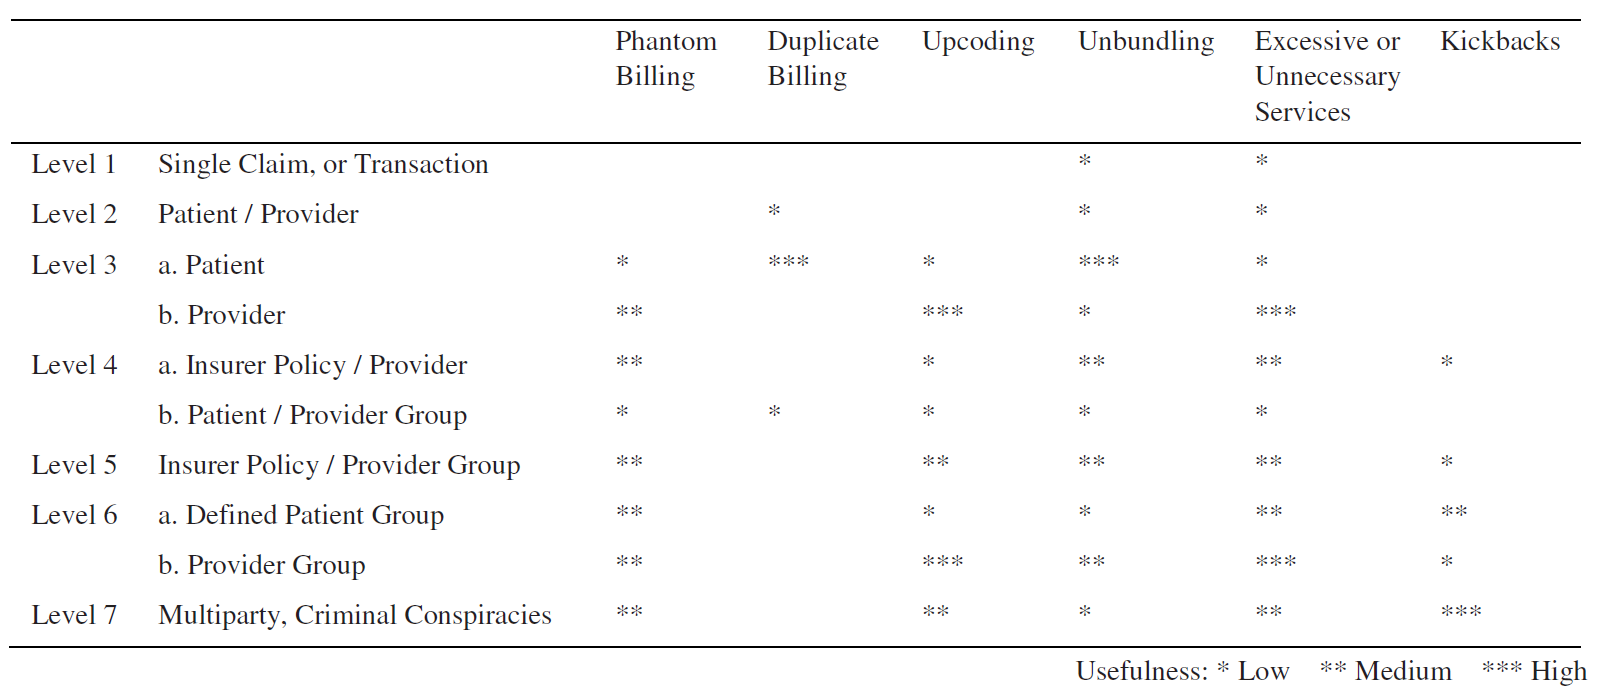
\includegraphics[scale=0.60]{images/TypesofFraud.png}
\end{table}


\end{document}
